% Simulating measurements of the main station Zurich

\noi The experiments were only analyzed visually by judging how well our model could cope with the given task and how it compared to the real observations. In figure \ref{fig:ex5picture}, one final situation for each run is given as an example.\\

\begin{figure}[h!]
	\centering
		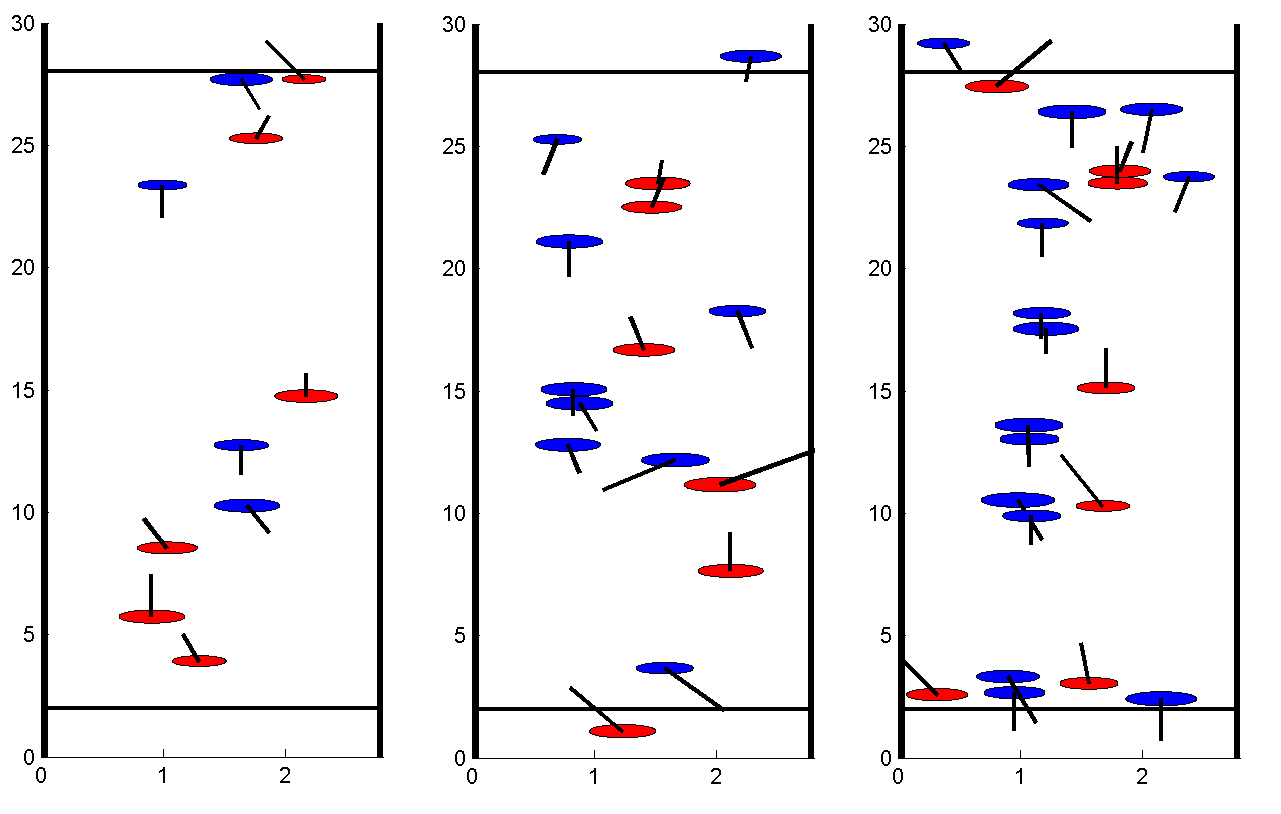
\includegraphics[width=0.90\textwidth]{pictures/ex5picture.png}
	\caption{Exemplary pictures for the simulation of the long narrow hallway in the Zurich main station. Red agents are walking up and blue down, the black line denotes the actual velocity vector with its angle and length. The left was done with flux densities of 0.12/0.17, the middle with 0.34/0.275 and the right with 0.6/0.5 after a simulation time of 180 seconds. In all investigated situations, the agents managed to cross the hallway without significant hindrance from other agents.}
	\label{fig:ex5picture}
\end{figure}

\noi For the first simulation series with a low people flux, the agents had no problems and could avoid collisions/walking into each other easily. This is in accordance with the observations.\\

\noi For the second simulation series with a medium people flux, the agents had little problems crossing the hallway. The stop-and-go of the observation was only rarely seen, suggesting that the logic behind our model is actually quite good.\\

\noi In the third simulation series with a high people flux, the agents had to stop sometimes while getting on the other side. But overall they could cope quite well with the task and the frequency of agents bumping into each other was quite slow and definitely in the same range as in real situations. Sometimes a small lane formation could be observed.\\

\noi We can say that our simulation worked well on the measured quantities. Of course, in reality, when jams start, there will be more side effects as people pushing, turning around, or trying to walk another way, but for a straightforward walk, our simulations mirrors the reality nicely.
